\documentclass[a4paper]{article}

%% Language and font encodings
\usepackage[english]{babel}
\usepackage[utf8x]{inputenc}
\usepackage[UTF8]{ctex}
\usepackage[T1]{fontenc}
%
%% Sets page size and margins
\usepackage[a4paper,top=3cm,bottom=2cm,left=3cm,right=3cm,marginparwidth=1.75cm]{geometry}

%% Useful packages
\usepackage{amsmath}
\usepackage{graphicx}
\usepackage[colorinlistoftodos]{todonotes}
\usepackage[colorlinks=true, allcolors=blue]{hyperref}
\usepackage[numbers,sort&compress]{natbib}
\newcommand{\upcite}[1]{\textsuperscript{\cite{#1}}}
\newcommand{\topcaption}{%
    \setlength{\abovecaptionskip}{0pt}%
    \setlength{\belowcaptionskip}{10pt}%
    \caption}   % 表格上标题修改
%_____________________________________________
\title{Solve TSP With Machine Learning}
\author{周宇轩\ 1800013075\\黄海晨\ 1800013072\\王帅\ 1800012995}
\date{}

\begin{document}

\maketitle

%_____________________________________________
\begin{abstract}
        我们使用了神经网络与强化学习两种结构来得到TSP问题的近似解,并通过与贪心、近似比为1.5的传统算法进行比较估计结果的优劣来体现两种结构对于TSP问题的近似效果,最后简单分析效果不理想的原因。
\end{abstract}
%____________________________________________

\section*{Introduction}

由于近年兴起的深度网络在许多实际应用上取得了显著的效果,同时强化学习、迁移学习等新方式也展现出机器学习的更多可能。我们希望测试这些新方法在NP问题上的效果,通过建立神经网络与强化学习两种模型对经典的NPC问题TSP,即货郎问题的最优解进行近似。我们考察了两篇论文Pointer Networks与NEURAL COMBINATORIAL OPTIMIZATION WITH REINFORCEMENT LEARNING(两篇论文的原件附在文件夹当中),按照文中的架构进行的复现,并将复现的结果与传统方法比较。对于神经网络的建模,基于无法对每一个数据规模进行训练,采用了RNN将输入数据看作序列处理,利用seq2seq模型提取隐状态,同时通过attention机制得到相应的输出。对于强化学习的建模,我们将游走顺序看作策略,游走长度看作应当最小化的函数,利用已有的RNN网络估计期望长度进行强化学习。

\section*{Pointer Network}

Pointer Network采用seq2seq with attention模型,该模型基于普通的seq2seq模型,在实现中我们简单的使用双层LSTM为encoder输出隐藏状态,decoder使用下方的pointer-attention形式生成。在注意力层次方面,encoder、decoder的隐层为$(e_1,...,e_n)$和$(d_1,...,d_{m(P)})$,其中$n$为数据规模大小,而$m(P)$为根据问题类型与实例$P$所需要回答的长度,在TSP问题中$m(P) = n -1$,因为开头和结尾默认为1号节点。我们再定义如下变量:

$$u^i_j = v^T tanh(W_1e_j+W_2d_i)\ j\in (1,...,n)$$

$$a^i_j = softmax(u^i_j)\ j\in (1,...,n)$$

$$d'_i = \sum_{j=1}^n a^i_j e_j$$

其中softmax将$u^i$归一化为输入的"attention" mask,$v,W_1,W_2$为需要学习的参数,同时保持隐层的维度为512,最后需要将$d'_i,d_i$连接起来作为用于预测隐层状态与下一步的隐层计算。可以简单看出时间复杂度为$O(n^2)$。

下图为seq2seq结构图与attention机制图:

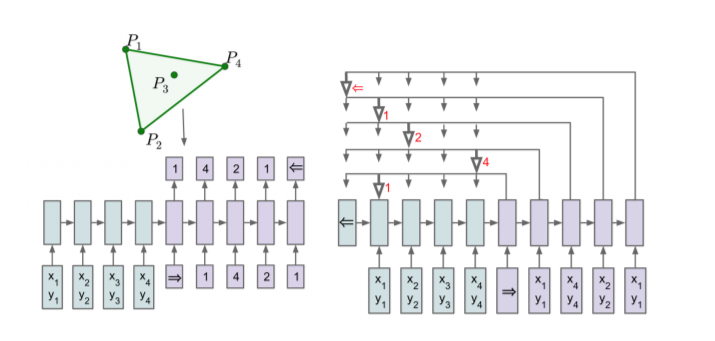
\includegraphics[]{../fig/pic1.png}

我们将在decoder第i步对前n个输入隐层的attention向量$a^i$归一化后的$u^i$向量看作一个概率分布,表示第i步输出关于输入n个点的概率分布,在其中挑选最大的作为第i步的输出。这个过程在训练时不会有问题,但在输出时可能会出现会有重复。

这里有两种解决方式:方式1为使用beam search,这样比每步贪心得到的解更优。方式2为改变网络结构,在网络前向过程中就对输出加以限制,维护一个mask,不允许选择已经选过的点(使其概率为零)。我们对于两种方法都进行了实验,二者的差异将在result中展现。

更近一步地,代码中具体参数为batch size=128,hidden units=512,learning rate=0.005,ADAM优化器,损失函数采用输出序列和最优解序列的交叉熵。



\section*{Reinforcement Learning}

上面我们用模型输出结果和已有的解的交叉熵作为损失函数,属于有监督学习,模型求解的质量理论上受限于训练数据集的质量,是在模仿之前的策略。而tsp问题目前并没有确定性的寻找最优解算法,因此我们也希望通过训练找到更优的策略,而不是模仿已有的策略。

考虑使用强化学习算法,下面给出强化学习的场景的符号描述:

定义状态集$S$,状态$s\in S$,这里$S$为$\left([0,1]\times[0,1]\right)^n\times\left(\{1,2,\dotsb,n\}\right)^2$上的集合,表示在$n$个点的图中的哪个位置,走到了第几步。

定义状态序列$\{s_0,s_1,\dotsb s_t\}$,和动作序列$\{a_0,a_1,\dotsb a_t\}$,其中$s_0$为初始状态,$s_t$为在时刻$t$处于的状态,$a_t$为在时刻$t$采取的行动,且满足$a_t\sim \pi\left(s_{t}\right)$,意为在状态$s_t$时,按照策略$\pi$的概率分布采取行动$a_t$,这里$a_t$即为在当前点前往下一个点的动作

定义每一步行动的回报$R\left(s_t,a_t\right)$,则这里一步的回报为第$t$个点到第$t+1$个点的距离。

目标函数有多种定义方式,如初始状态到终止状态的回报和,或是动作序列每个状态到终止状态的回报和平均值等,这里我们采用初始状态到终止状态的回报和来定义,即
$$J=E\left(\sum_t\gamma^tR\left(s_t,a_t|\pi\right)\right)$$.
其中$\gamma$是衰减因子,这里我们取$\gamma=1$,则事实上目标函数可写成$J\left(s\right)=E_{a\sim \pi\left(s\right)}\left(L\left(a|s\right)\right)$,其中$s$仅表示图中点的信息,$a$为按照策略$\pi$选择的排列,$L\left(a|s\right)$即为按这个排列走出的路径长。

我们的目标是最小化目标函数。

我们依然采用Pointer-Network来给出策略$\pi$(即在每个时刻选择下一个点的概率),令$\theta$为网络参数,则有
$$J\left(\theta |s\right)=E_{a\sim \pi_\theta\left(s\right)}\left(L\left(a|s\right)\right)$$.
则根据策略梯度定理,有
$$\nabla J\left(\theta|s\right)\approx E_{a\sim \pi_\theta\left(s\right)}\left(L\left(a|s\right)\nabla_\theta\log \pi_\theta\left(a|s\right)\right). $$
这里$\pi_\theta\left(a|s\right)$为参数$\theta$下按策略$\pi_\theta$在图$s$得到排列$a$的概率。

采用蒙特卡洛方法对图分布$s\sim S$进行采样(就是在$[0,1]\times[0,1]$上随机生成图),并在选择输出排列时按概率分布$p_\theta$进行采样,则可得到对$J\left(\theta\right)$的无偏估计
$$\nabla J\left(\theta\right)\approx \dfrac{1}{B}\sum_{i=1}^BL\left(a_i|s_i\right)\nabla_\theta\log \pi_\theta\left(a_i|s_i\right). $$
如果样本对期望的方差过大,由于我们训练时每步都更新参数,可能导致模型难以收敛到最优区域。考虑加入baseline function$\ b\left(s\right)$,用来减小更新参数时梯度的方差,则式子改写为:
$$\nabla J\left(\theta\right)\approx \dfrac{1}{B}\sum_{i=1}^B\left(L\left(a_i|s_i\right)-b\left(s_i\right)\right)\nabla_\theta\log \pi_\theta\left(a_i|s_i\right). $$
加入$b\left(s\right)$对梯度的期望没有影响。这是因为
\begin{align*}
  E_{a\sim \pi_\theta\left(s\right)}b\left(s\right)\nabla_\theta\log \pi_\theta\left(a|s\right)&=\sum_{a\in \pi_\theta\left(s\right)}\pi_\theta\left(a|s\right)b\left(s\right)\nabla_\theta\log \pi_\theta\left(a|s\right)&\ \\
  &=b\left(s\right)\sum_{a\in \pi_\theta\left(s\right)}\pi_\theta\left(a|s\right)\dfrac{\nabla_\theta\pi_\theta\left(a|s\right)}{\pi_\theta\left(a|s\right)}\\
  &=b\left(s\right)\sum_{a\in \pi_\theta\left(s\right)}\nabla\pi_\theta\left(a|s\right)\\
  &=b\left(s\right)\nabla1=0.
\end{align*}
考虑选取怎样的$b\left(s\right)$能使方差更小。考虑$b\left(s\right)$对方差的影响:
\begin{align*}
  &D_{a\sim \pi_\theta\left(s\right)}\left(\sum_{i=1}^B\left(L\left(a_i|s_i\right)-b\left(s_i\right)\right)\nabla_\theta\log \pi_\theta\left(a_i|s_i\right)\right)&\ \\
  =&E_{a\sim \pi_\theta\left(s\right)}\left(\left(\sum_{i=1}^B\left(L\left(a_i|s_i\right)-b\left(s_i\right)\right)\nabla_\theta\log \pi_\theta\left(a_i|s_i\right)\right)^2\right)-E_{a\sim \pi_\theta\left(s\right)}^2\left(\sum_{i=1}^B\left(L\left(a_i|s_i\right)-b\left(s_i\right)\right)\nabla_\theta\log \pi_\theta\left(a_i|s_i\right)\right)\\
  \approx&E_{a\sim \pi_\theta\left(s\right)}\left(\left(\sum_{i=1}^B\left(L\left(a_i|s_i\right)-b\left(s_i\right)\right)\nabla_\theta\log \pi_\theta\left(a_i|s_i\right)\right)^2\right)\ \ \left(1\right)\\
  \approx&\sum_{i=1}^BE_{a\sim \pi_\theta\left(s\right)}\left(\left(L\left(a_i|s_i\right)-b\left(s_i\right)\right)^2\right)\sum_{i=1}^BE_{a\sim \pi_\theta\left(s\right)}\left(\nabla_\theta\log \pi_\theta\left(a_i|s_i\right)^2\right)\ \ \left(2\right)\\
  \approx&\sum_{i=1}^BE_{a\sim \pi_\theta\left(s\right)}\left(\left(L\left(a_i|s_i\right)-b\left(s_i\right)\right)^2\right)\ \ (3).
\end{align*}
这里(1)步用到之前证明的$b\left(s\right)$对期望无影响,故我们可以不考虑期望的平方项;(2)步假设各样本之间、几个参数之间都具有独立性;(3)步去掉了与$b\left(s\right)$无关的项。

很明显,$b\left(s\right)$对方差的影响项$\sum_{i=1}^BE_{a\sim \pi_\theta\left(s\right)}\left(\left(L\left(a_i|s_i\right)-b\left(s_i\right)\right)^2\right)$是一个均方误差的形式,故我们选择$b\left(s\right)=E_{a\sim \pi_\theta\left(s\right)}L\left(a_i|s_i\right)$时能将这一项的值降到最小。

下面考虑估计$ E_{a\sim \pi_\theta\left(s\right)}L\left(a_i|s_i\right)$.

一种方法较为简单,采用指数移动平均的形式,即把每个样本$s_i$在经过网络后得到的结果$L\left(a_i|s_i\right)$进行加权平均作为估计,早期的结果权重会指数衰减,总的估计可以采用以下式子计算:
$$EMA_t=
\begin{cases}
  L\left(a_t|s_t\right), & t=1 \\
  \left(1-\beta\right)L\left(a_t|s_t\right)+\beta EMA_{t-1}, & t>1
\end{cases}$$
其中$\beta$为衰减因子,衡量衰减速度的快慢。

另一种方式是用一个另外的网络对$ E_{a\sim \pi_\theta\left(s\right)}L\left(a_i|s_i\right)$进行估计,这个网络称为critic network,之前的pointer network称为actor network,它的结构如下:
\begin{enumerate}
\item 首先是一个与actor network中encoder类似的LSTM RNN
\item 接另一个LSTM单元,将encoder的最后一个隐层向量作为初始隐状态,每次令其经过单元并计算之前attention机制所述的context,将context作为下一步的输入。这个过程重复$P$次
\item 让最后的隐层向量经过$d*d$全连接——ReLU——$d*1$全连接层,得到最终的估计值。$d$为隐层向量维数
\end{enumerate}
损失函数选用估计值与当前的解的均方误差MSEloss.
\\

则整个训练的过程为:
\begin{enumerate}
\item 获取数据
\item 数据经过actor network得到当前解

  解的选取方式:不使用贪心策略,根据当前的概率分布选择,即采样(可以用pytorch中的multinomial函数实现),并且选择过程中对选项加mask(之前提到的第二种写法),从而保证解是合法的
\item 用critic network(或者指数移动平均)对解的期望长度进行估计,得到baseline function
\item 计算actor network的loss并bp.
\item 计算critic network的loss并bp(若使用指数移动平均则没有这一步).
\end{enumerate}

\section*{Data and Baseline}

训练数据中的输入为为在$[0,1]×[0,1]$上的大小为$n$的随机点集,输出为大小为开头为1结尾为1,同时前$n$个数组成$n$排列的$n+1$个数。

下面讨论关于TSP结果的baseline,训练数据中所有大小为5,10训练数据输出均为最优解,计算最优解使用的是时间复杂度为$O(n^22^n)$的动态规划算法,具体地定义$dp[S][i]$为当前经过顶点集合为$S$,结束点为$i$时最短路径,每次枚举下一步节点进行转移。

训练数据中所有大小为20训练数据输出为近似解,这里采用了两种算法。算法1为贪心算法,每次走向离当前节点最近的节点;算法2为近似比为1.5的算法,先在图中求最小生成树,再对树中的所有奇数节点使用一般图最小权匹配,在树中加入匹配边,最后通过Fleury算法求欧拉回路,在该欧拉回路基础上得到一个哈密尔顿回路,算法时间复杂度为$O(n^3)$。在下方的result中会将贪心与近似算法作为baseline。

\section*{Result}

下表为各个算法对整体测试数据求出的平均长度:

\begin{tabular}{c|c|c|c|c}
    $n$ & PtrNet & Reinforcement & Greedy & Approximate  \\ \hline
    5 & 2.28 & - & - & - \\
    10 & 3.3 & - & - & - \\
    20 & 6.57 & 4.27 & 4.49 & 4.20 \\
    40 & 11.8 & 6.16 & 6.40 & 5.78 \\ \hline
\end{tabular}

由于当$n=5,n=10$时,PtrNet得到的平均值最优解平均值为1.03倍与1.15倍,均为非常不错的近似比。

可以发现随着$n$的变大,PtrNet与RL得到的结果不断增大,且没有达到一个稳定的近似比,对于一个近似算法而言并不优秀。但对于PtrNet使用强化学习的确取得了不错的效果。总的来说,强化学习的效果比贪心更好,但差于近似比为1.5的近似算法。

详细的训练结果在报告最后

\section*{Summary}

本文采用了PtrNet与强化学习两种方法对TSP问题进行了尝试,取得了比普通贪心优秀的结果,但仍然比不上传统近似算法。其中非常有趣的一点是贪心、PtrNet与RL的复杂度均为$O(n^2)$,而近似算法的复杂度为$O(n^3)$,在实验中复杂度更高的算法取得了更优秀的结果,尽管神经网络在拟合函数方面非常强,但还是稍逊一筹,这让我们对于NP问题多项式算法的近似能力是否有限,而例如$O(n),O(n^2),O(n^3)$等多项式时间的算法的最优近似能力是否越来越强产生了疑惑。而对于利用神经网络作为近似算法的下一步很可能需要加深网络提高算法复杂度,同时也需要加强训练方法,来保证深度网络的效果。

\begin{thebibliography}{99}
\bibitem{ref1}Oriol Vinyals, Meire Fortunato and Navdeep Jaitly, Pointer Networks, arXiv preprint arXiv:1506.03134
\bibitem{ref2}Irwan Bello, Hieu Pham, Quoc V. Le, Mohammad Norouzi and Samy Bengio, NEURAL COMBINATORIAL OPTIMIZATION WITH REINFORCEMENT LEARNING, arXiv preprint arXiv:1611.09940
\bibitem{ref3}https://danieltakeshi.github.io/2017/03/28/going-deeper-into-reinforcement-learning-fundamentals-of-policy-gradients/
\bibitem{ref4}https://github.com/higgsfield/np-hard-deep-reinforcement-learning
\bibitem{ref5}https://github.com/pemami4911/neural-combinatorial-rl-pytorch
\end{thebibliography}

\section*{Detail}

以下为普通Pointer-Network的两种实现方式训练中的loss和对训练集的平均解长度对比:

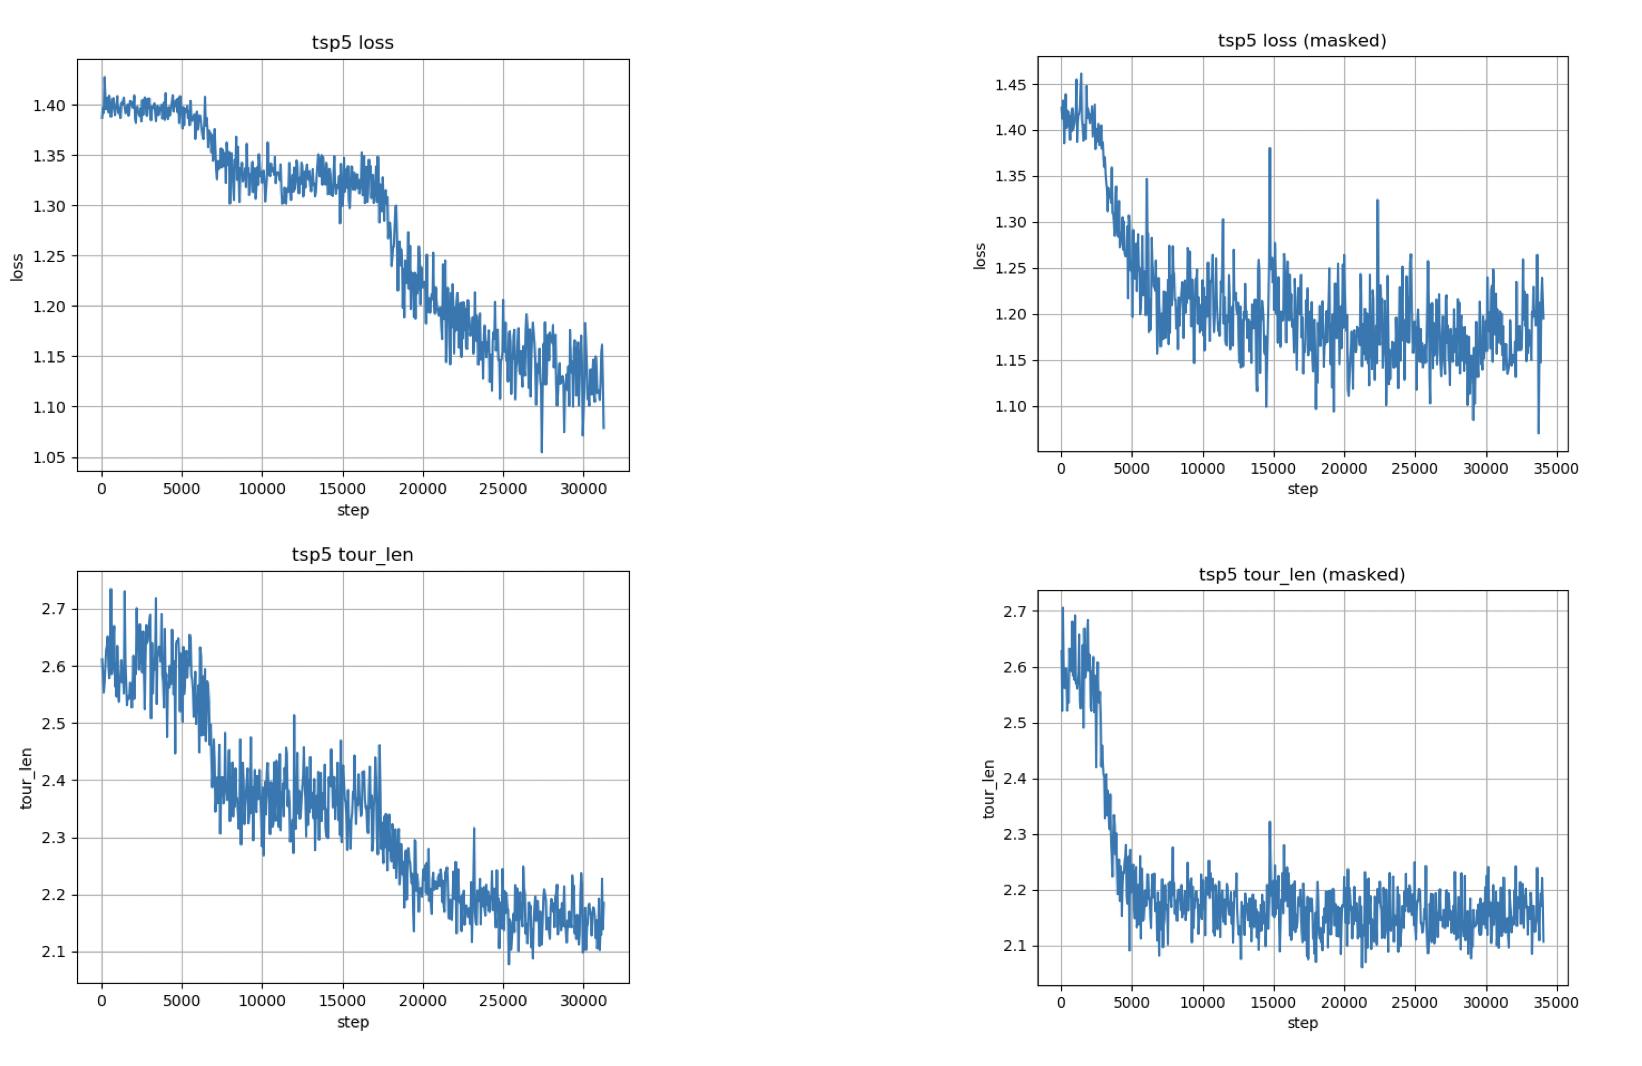
\includegraphics[width=\textwidth]{../fig/pic2.png}

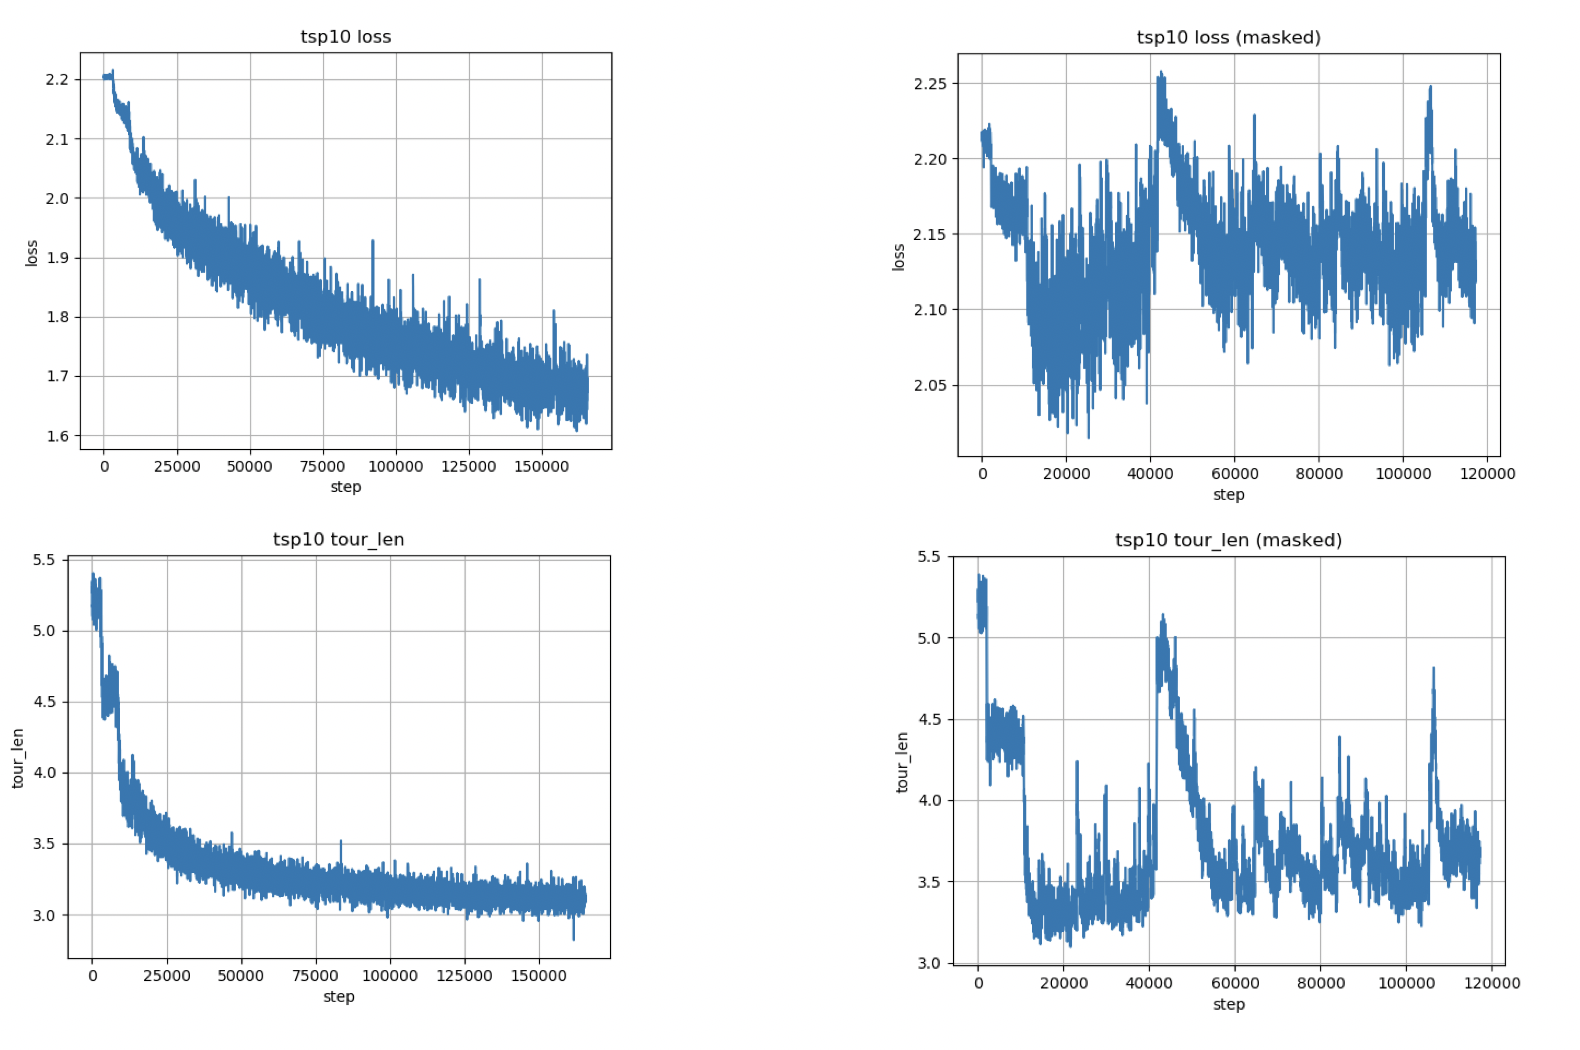
\includegraphics[width=\textwidth]{../fig/pic3.png}

可以看到第二种实现方式loss一开始下降很快,这里我们认为是因为第一种实现方式要额外学习怎样生成排列;但第二种实现方式后期的表现十分令人费解,解的质量和loss都没有收敛的意思,所以我们最终还是采用了第一种实现方式,其数据在各方面上看都比较符合常理。

以下为普通Pointer-Network的第一种实现方式训练数据规模为20的图过程中的loss和对训练集的平均解:

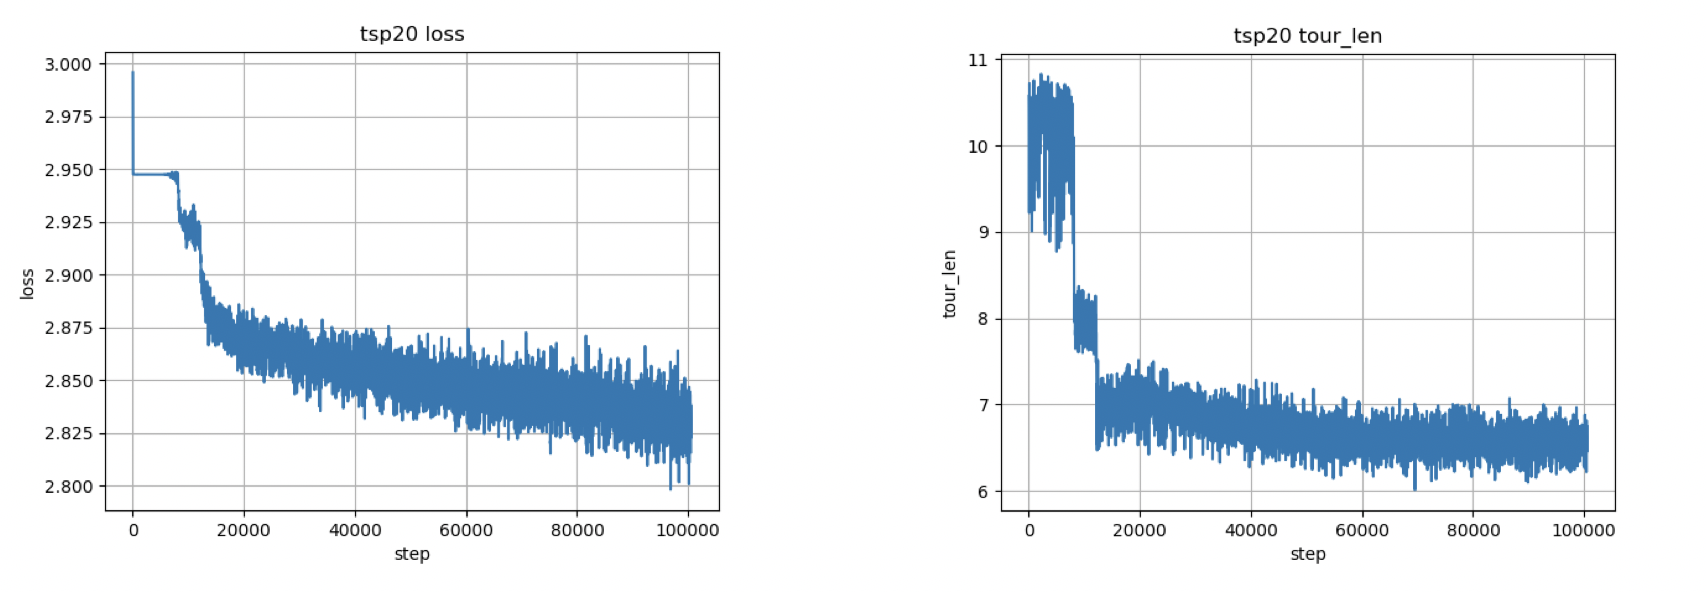
\includegraphics[width=\textwidth]{../fig/pic4.png}

以下为强化学习训练数据规模为20和40的图过程中对训练集的平均解:

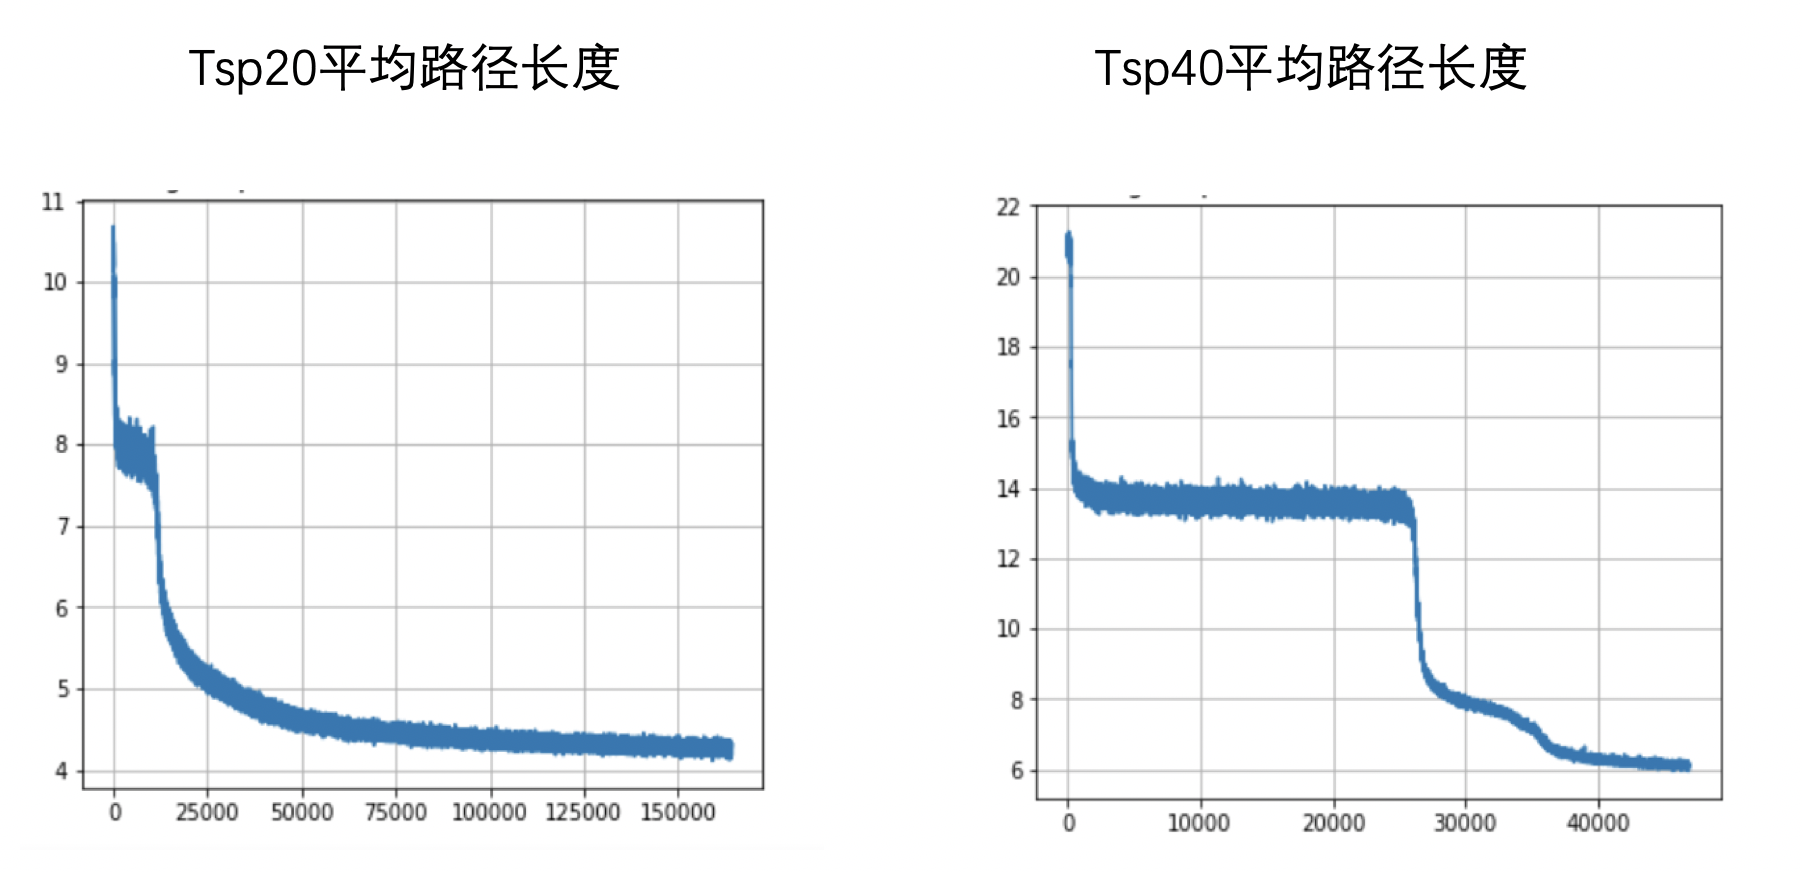
\includegraphics[width=\textwidth]{../fig/pic5.png}



\end{document}